\documentclass[10pt,a4paper,oneside]{article}
\usepackage[utf8]{inputenc}
\usepackage[english]{babel}
\usepackage{amsmath}
\usepackage{amsfonts}
\usepackage{amssymb}
\usepackage{graphicx}
\usepackage[left=2cm,right=2cm,top=2cm,bottom=2cm]{geometry}
\author{Hazem Hussien}
\title{Fruit Ninja Game Report}
\begin{document}

\maketitle

\newpage
\begin{samepage}
\section{Design Explanation}
I used MVC in the design of this app,I have 2 views , one for the main menu and another one for the actual game , and each one has its controller that it's communicating with.

\vspace{10px}

I have made 4 fruit classes(Watermelon,Lemon,pineapple,Banana) and 2 Different Bomb types (Death Bomb and Life Bomb) that all extend the GameObject class.

I have only one model class GameModel that is responsible for managing the data and sending it to the controller so that it can pass it to view.

\section{Snapshots Of GUI}
\vspace{15px}
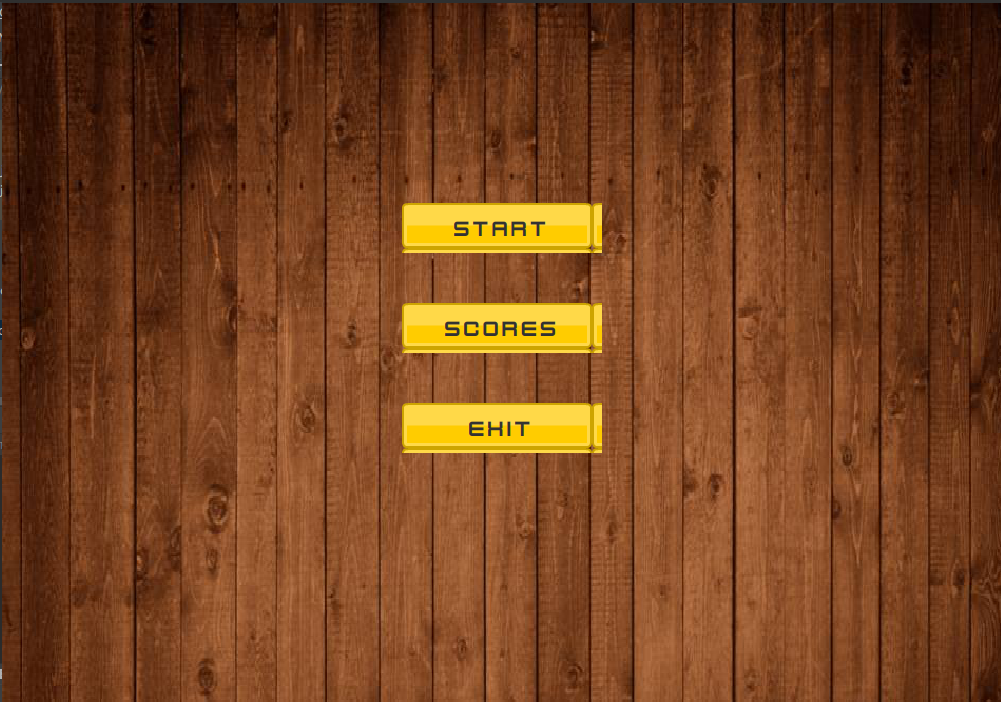
\includegraphics[width=15cm,height=14cm,keepaspectratio]{gui1.png}

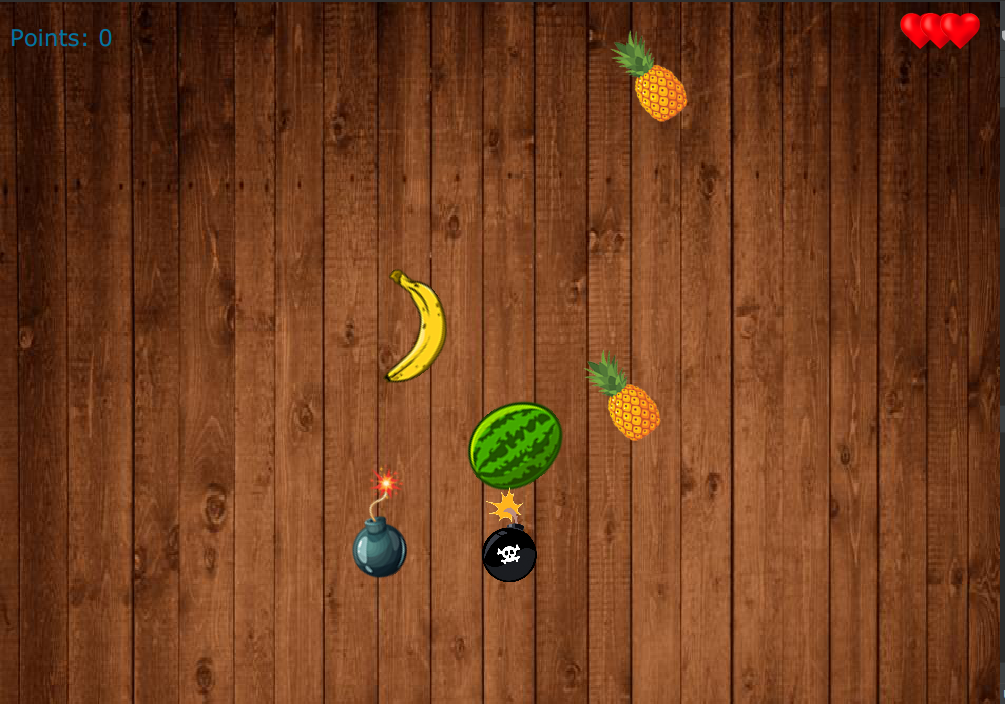
\includegraphics[width=15cm,height=14cm,keepaspectratio]{gui2.png}

\end{samepage}

\section{Design Pattern Used}

I only used three design patterns
1)Factory Method Pattern : to encapsulate the creation of my fruits and bombs objects


2)Decorator Pattern : to Add extra points to some fruits and other feartures like "Add Life"


3)Singleton Pattern : used it to make sure that only one instance of my ViewManager is created as i don't want mutiple instances of it by accident. 

\section{How to use the application}
To use the app all you have to do is press start once the application loads. 

\end{document}